\chapter{Results}%
\label{chap:results}
\textit{This chapter presents the test results that test and challenge the proposed method.  The randomization tests, which additionally test the influence of the \ac{kgraph} and test taken including and excluding the \ac{kgraph}. The test results provide evidence that supports the effectiveness of the proposed method. This chapter starts by introducing \textbf{method metrics} that indicate how a task has been executed by the proposed method in \Cref{sec:proposed_method_metrics}. A comparison is made with the state-of-the-art methods in \Cref{sec:compare_with_related_papers}. \bs}

\paragraph{The Simulation Environment}
Testing in a simulation environment has been done using the URDF Gym Environment~\cite{spahn_urdfenvironment_2022}, a 100\% python environment build upon the PyBullet library~\cite{coumans_pybullet_2016}. The code created during the thesis can be found on \href{https://gitlab.tudelft.nl/airlab-delft/msc_projects/msc_gijs_groote}{GitLab} and \href{https://github.com/GijsGroote/semantic-thinking-robot}{GitHub}. Experiments ran on standard TU Delft laptop: HP ZBook Studio x360 G5, running OS:~Ubuntu 22.04.1 LTS x86\_64, CPU: Intel i7-8750H (12) @ 4.100GHz, GPU: NVIDIA Quadro P1000 Mobile.\bs
The simulation environment provides many different robots, 2 simple robots are selected to perform tests, they are displayed in \Cref{fig:example_robots}, and various objects are displayed in \Cref{fig:example_objects}.

\section{Proposed Method Metrics}%
\label{sec:proposed_method_metrics}
The results are measured in method metrics, not to be confused with the monitoring metrics in \Cref{sec:monitoring_metrics} or the edge metrics in \Cref{subsec:edge_metrics}. The results are interesting, but most interesting is the progression of the method metrics over time. As will be shown, the effect of learning can be measured by investigating and tracking the method metrics over time. Furthermore, the method metrics will be used to compare the proposed method to relative state-of-the-art papers. First, the method metrics are presented in~\Cref{table:proposed_method_metrics} with corresponding argumentation on the relevance of the metric.\bs

\noindent
\begin{table}[H]
\centering
\begin{tabular}%
  {>{\raggedright\arraybackslash}p{0.25\textwidth}%
   >{\raggedright\arraybackslash}p{0.65\textwidth}}
Total Average\newline \acl{PE} & The total average \ac{PE} is created by averaging over every hypothesis' average \ac{PE} in a \ac{hgraph}. Since the \ac{PE} is high when unexpected behaviour occurs, seeing the total average \ac{PE} lower would indicate the robot encounters less unexpected behaviour, indicating the robot is learning.\\
% Total Average\newline \acl{TE}& The total average \ac{TE} is created by averaging over every hypothesis' average \ac{TE} in a \ac{hgraph}. Seeing the total average \ac{TE} lower over time would indicate the robot is selecting better suitable controllers and system models, indicating the robot is learning.\\
% Final positions and\newline displacement errors & The final position and displacement error is a metric which how a controller performs. This thesis does not create or investigate controllers, but it is interesting to see why different controllers are preferred for different objects. The final position and displacement error could be the cause.\\
The ratio between the number of hypotheses and the number of tasks & Expected is that whilst learning system models, the hypothesis created will be more effective. Thus the ratio between the total number of hypotheses and the total number of tasks is expected to lower with new knowledge.\\
The ratio between the number of successful and the number of total edges in \ac{kgraph} & When the \ac{kgraph} improves recommending a controller and system model, the ratio between successful edges and total edges is expected to increase because, with better recommendations, more edges will be completed.\\
task completion time =\newline run time + planning time& If equal tasks are given multiple times, the total task completion time should drop pretty drastically. Multiple factors help to lower the task completion time, firstly system identification has to be performed only once, and there is no need to lose time on redoing system identification. Secondly, the \ac{hgraph} is expected to improve generated hypothesis, or better said, the same mistake should not be made multiple times, resulting in fewer failing hypotheses and lowering task completion time.\\
\end{tabular}
\caption{Proposed method metrics used to compare the proposed method with the state-of-the-art methods.}\label{table:proposed_method_metrics}
\end{table}

Three system models are used for testing. The goal of this thesis is not to find optimal control, or to model the environment very accurately. The goal is to select the best combination of controller and system model in the available set of controllers and system models. Only a short textual description of the available system models is provided below.\bs
 

\noindent
\begin{table}[H]
\centering
\begin{tabular}%
  {>{\raggedright\arraybackslash}p{0.25\textwidth}%
   >{\raggedright\arraybackslash}p{0.65\textwidth}}
\textit{lti-drive-model} & A second order \ac{LTI} model that can be used by both the \ac{MPC} and the \ac{MPPI} drive controller. The next robot configuration is based on the current configuration and system input in \gls{x} and \gls{y} direction. \\
\textit{nonlinear-push-model-1} & A nonlinear model describing the next object configuration in \gls{x} and \gls{y} direction and the orientation \gls{theta} based on the current configurations of the robot, the object and on the robot inputs in \gls{x} and \gls{y} direction.\\
\textit{nonlinear-push-model-2} & A nonlinear model describing the next object configuration in \gls{x} and \gls{y}, and the object configuration in \gls{x} and \gls{y} direction based on the current configurations of the robot, the object and on the robot inputs in \gls{x} and \gls{y} direction.\\
\end{tabular}
\caption{Available drive and push system models used for testing.}\label{table:available_system_models}
\end{table}


% \todo[inline]{make the environment that shows learning object is unmovable}
% \begin{figure}[H]
%     \centering
%     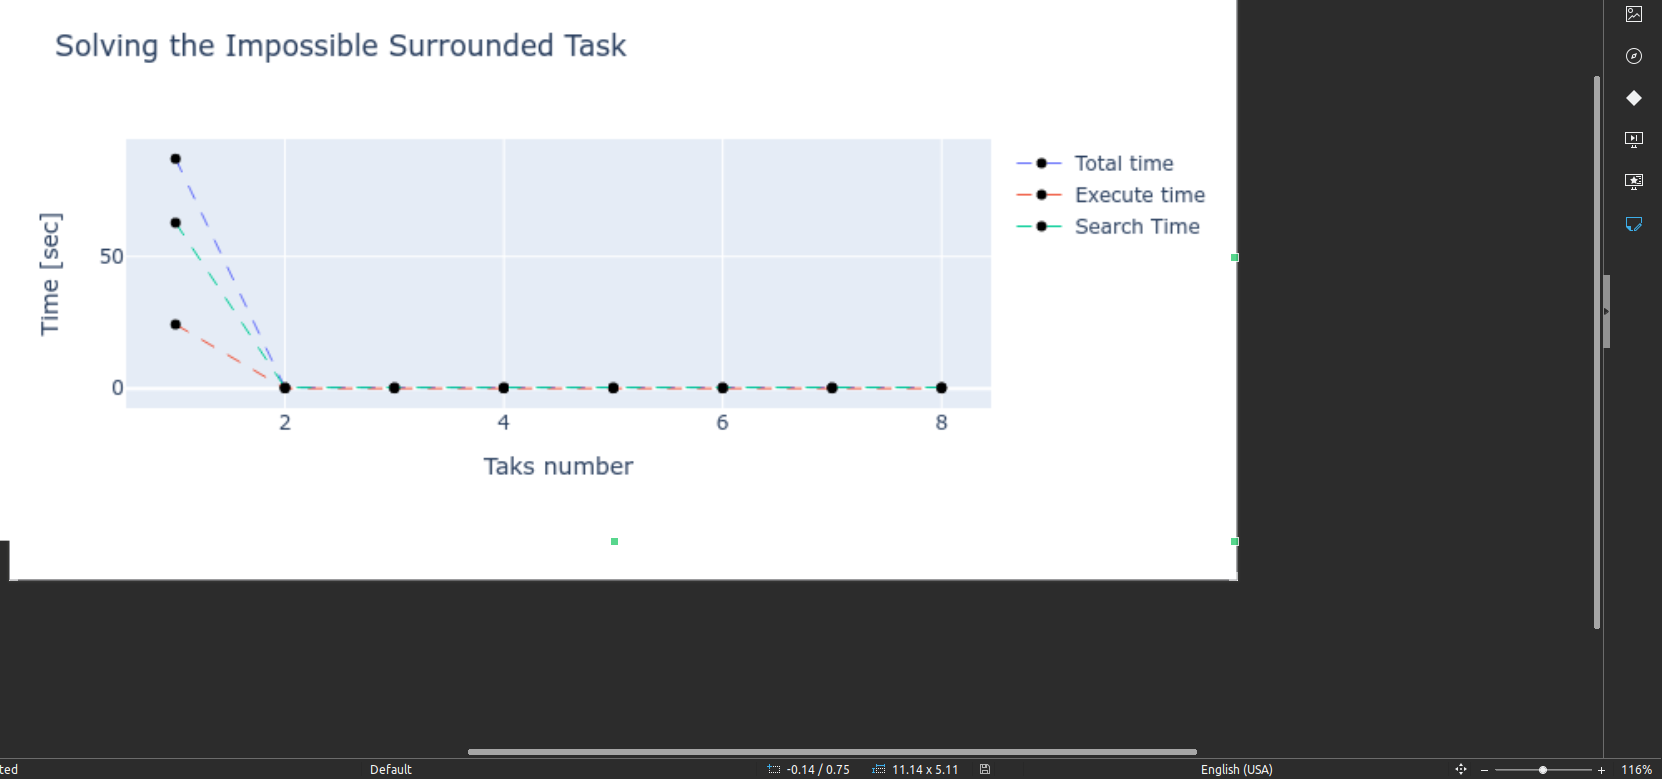
\includegraphics[width=5cm]{figures/results/execution_time_move_2}
% figures/figures/figures/figures/
%     \caption{}%
%     \label{}
% \end{figure}


% \section{Benchmark Tests}%
% \label{sec:benchmark_tests}
% Three benchmark test are presented, starting with the blockade task. A large part of the proposed method is system identification, for testing however no system identification is performed. Instead, several hard-coded system models are used, and the \ac{kgraph} finds which system model is the best choice for an object over time. Where the best choice is defined using the edge metrics discussed in \Cref{subsec:edge_metrics}. The hard-coded system models are not opting for modelling the drive or push model as accurately as they possibly can, thus severe model mismatch should be expected. Such model mismatch is no issue, to complete a subtask stable closed-loop control is required, when an edge parameterization is unable to provide closed-loop stable control, the edge will fail because a fault will be detected. To answer the research question, improvement over time should be made. Gaining such improvement does not require accurate system models, time spend improving the hand-coded system models does thus not change the result.\bs
%
%
% \paragraph{Blockade} In the blockade environment the robot is tasked with placing a box in a target position that is blocked by a cylinder object.\bs
% \begin{figure}[H]
%     \centering
%     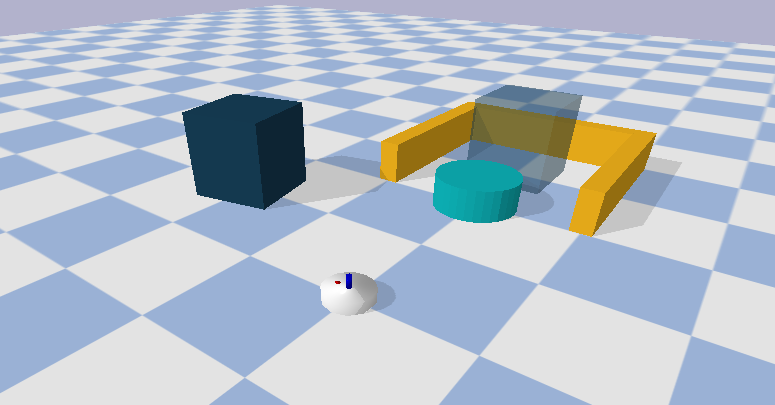
\includegraphics[width=0.9\textwidth]{figures/tests/blockade}
%     \caption{The blockade environment with the target ghost position for the blue box. The green walls are unmovable whilst both the blue box and cylinder are movable.}%
%     \label{fig:benchmark_blockade}
% \end{figure}
%
% The blockade task neatly shows that the \ac{halgorithm} uses the backward search technique. First, the \ac{halgorithm} plans to push the box directly to the target position, then it realizes a blocking object must first be moved to free the path. It makes the mistake of pushing the unmovable wall, then it succeeds in pushing the movable cylinder out of the way. The \ac{kgraph} then ensures that this mistake will not occur again because is remembered that the wall is immovable. Over time the \ac{kgraph} indicates that it prefers to use the \ac{MPPI} controller with the nonlinear-push-model-2 to push both the box and the cylinder object. Converging to this conclusion improves the method metrics for the task as can be seen in \Cref{fig:results_blockade}\bs
%
% \todo[inline]{is nonlinear-push-model-2 still the preferred model after testing??}
%
% \begin{figure}[H]
%     \centering
%     
\includegraphics[width=0.9\textwidth]{figures/tests/404_not_found}
%
%     \caption{Some tests are still under development for the blockade environment}%
%     \label{fig:results_blockade}
% \end{figure}
% \todo[inline]{Test to create results for running the blockade environment, and input into above 404 not found}
%
% \paragraph{Swap}
% In the swap environment the robot should swap the locations of the 2 objects in the environment.\bs
%
% \begin{figure}[H]
%     \centering
%     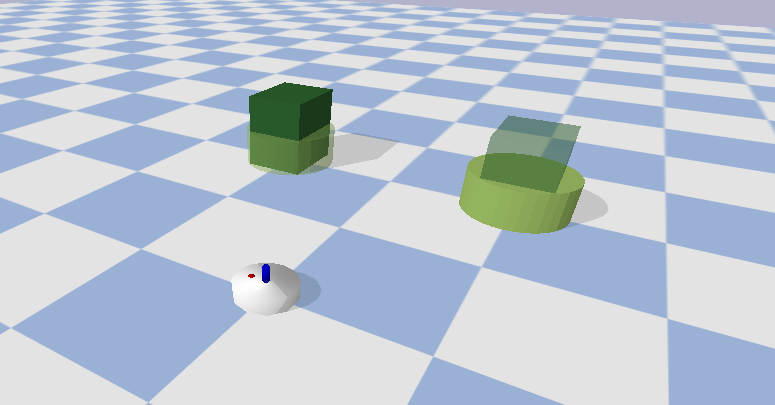
\includegraphics[width=0.9\textwidth]{figures/tests/swap}
%     \caption{The swap environment, the robot is tasked with swapping the positions of the cylinder and the box.}%
%     \label{fig:benchmark_swap}
% \end{figure}
% The swap task shows that the \ac{halgorithm} can handle overlapping subtasks. The \ac{halgorithm} handles a single subtask at a time and randomly selects which subtask to handle next. The result for the swap task is that first, the robot will place the box on the location of the cylinder. The cylinder is blocking the path and is thus pushed to free the path, then the robot drives back to the box to push the box to its target position. The cylinder can directly be pushed toward its target position, because there is a free path, and the task is successfully completed. By manual inspection, this is the most efficient action sequence to complete the swap task. But there is an assumption because the initial environment has a distance between the robot and box (robot-box distance), and robot and cylinder (robot-cylinder distance) that is equal. If the initial robot-box distance is greater than the initial robot-cylinder distance, it would be more efficient to first drive toward the cylinder because that distance is smaller. The selection of subtask is random, thus there is a 50\% chance that the robot selects a subtask resulting in driving more than is necessary to complete the swap subtask.\bs
%
% \begin{figure}[H]
%     \centering
%     
\includegraphics[width=0.9\textwidth]{figures/tests/404_not_found}
%     \caption{Some tests are still under development for the swap environment}%
%     \label{fig:results_swap}
% \end{figure}
%
% \todo[inline]{Test to create results for running the swap environment}
%
% \paragraph{Surrounded} In the surround environment the robot has to learn which box is movable to escape the enclosure of boxes.\bs
% \begin{figure}[H]
%     \centering
%     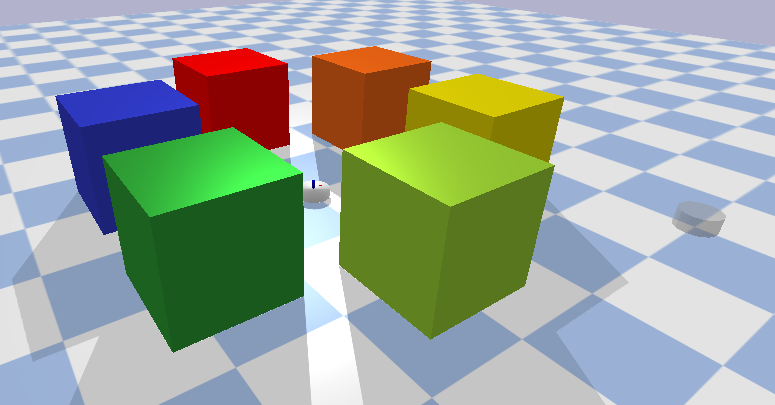
\includegraphics[width=0.9\textwidth]{figures/tests/surrounded}
%     \caption{The surround environment, the robot is tasked with escaping the surrounding enclosure by driving to the target ghost position displayed on the right side in the figure. Every box objects is unmovable except the red box which is movable.}%
%     \label{fig:benchmark_surround}
% \end{figure}
% The surround task show that having and gaining environment knowledge can greatly improve task execution. Simply knowing if an object can be interacted with may lower task execution time drastically as can be seen in \Cref{fig:results_surround}.\bs
%
% \begin{figure}[H]
%     \centering
%     
\includegraphics[width=0.9\textwidth]{figures/tests/404_not_found}
%     \caption{Some test are still under development for the surround environment}%
%     \label{fig:results_surround}
% \end{figure}
%
% \todo[inline]{Test to create results for running the surround environment}

\section{Randomization}%
\label{sec:randomisation}
In the randomized environment, the robot is tasked to push a number of objects to a target location. The previous 3 benchmark tests are designed around the proposed method, meaning that these tests highlight the strong points of the \ac{halgorithm} but prevent the testing of the weak points of the proposed methods. Such bias can lead to false positives, which are undesired. The randomized environment provides a more unbiased result. The random environment does not deliver completely unbiased results because several parameters must be chosen to create and set up the random environment, which are.\\

\noindent
\begin{table}[H]
\centering
\begin{tabular}%
{>{\raggedright\arraybackslash}p{0.25\textwidth}%
>{\raggedright\arraybackslash}p{0.65\textwidth}}
The \textit{size of the grid} & in \gls{x} and \gls{y} direction.\\
The \textit{minimal and maximal size of objects} & A box will have sides with a length that lie in the specified range from minimal to maximal length. Cylinders will have a diameter and height that is within the specified range, additionally, cylinders are not higher than the radius of the cylinder to prevent cylinders from tipping over. \\
The \textit{maximal weight} & which is uniformly distributed for the environment objects, minimal weight is set by default to 0. \\
The \textit{number of unmovable and movable objects} & For every new object generated there is a 50\% chance it becomes a box and 50\% chance it becomes a cylinder, letting randomization determine the ratio between boxes and cylinders. \\
The \textit{number of subtasks in a task} & Which must be greater or equal to the number of movable objects. The task has feasible targets that lie in free space, and the path estimator discussed in \Cref{subsec:path_estimation} is used to determine the target configuration for objects. By creating configuration space for an object the target configuration is chosen to be in free space, and then path estimation is used to determine if an object can reach the target configuration from its initial configuration.
\end{tabular}
\end{table}

If the task is completed, a \textit{reshuffle} function reshuffles the objects in the environment, that is the object remain the same objects, but the objects receive a new initial position, and the subtask target configurations are renewed. The reshuffled environments can be seen in \Cref{fig:random_environment_reshuffle}.\bs

\begin{figure}[H]
    \centering
    \begin{subfigure}{\textwidth}
    \centering
    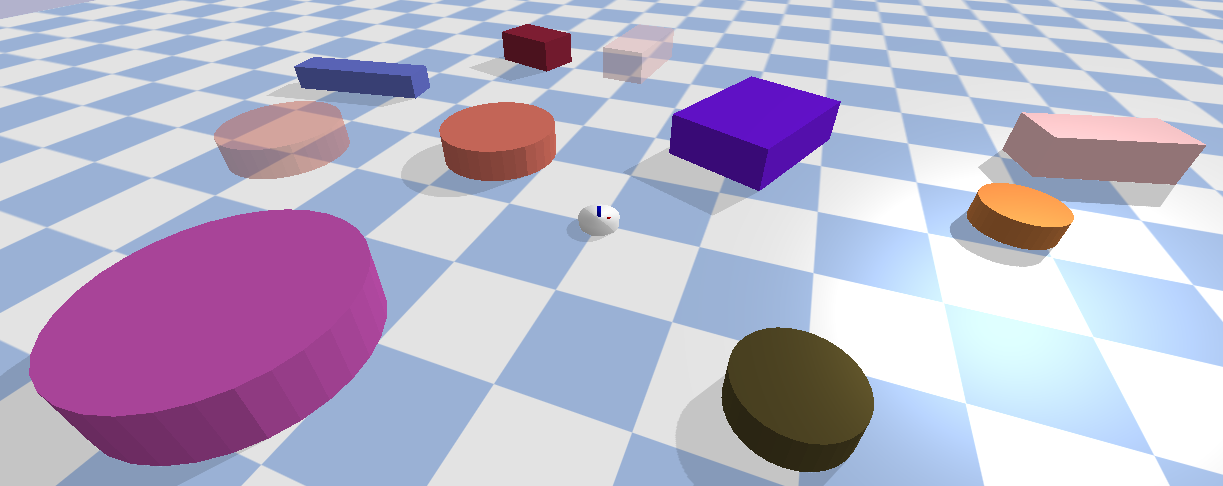
\includegraphics[width=0.9\textwidth]{figures/tests/random_1}
    \end{subfigure}

    \vspace{0.2cm}
    \begin{subfigure}{\textwidth}
    \centering
    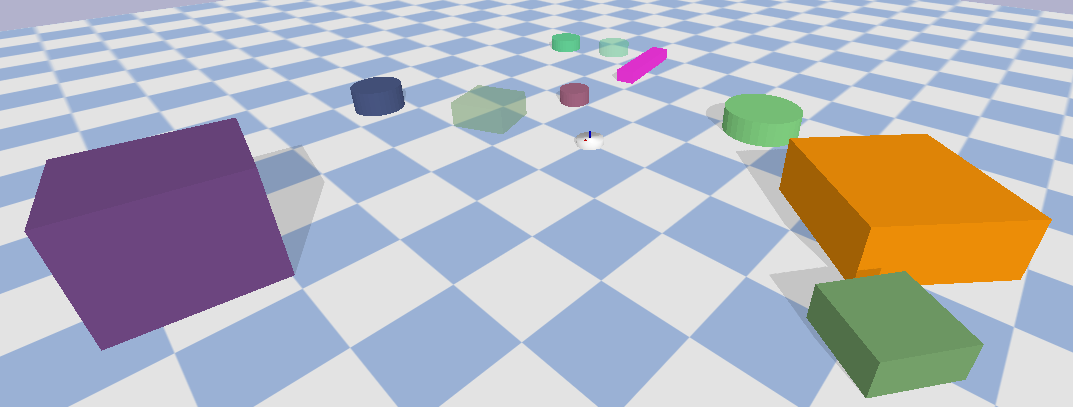
\includegraphics[width=0.9\textwidth]{figures/tests/random_2}
    \end{subfigure}
    \caption{Two random environments with 2 target ghost configurations for the task containing 2 subtasks.}%
    \label{fig:random_environnment}
\end{figure}

\begin{figure}[H]
    \centering
    \begin{subfigure}{.49\textwidth}
    \centering
    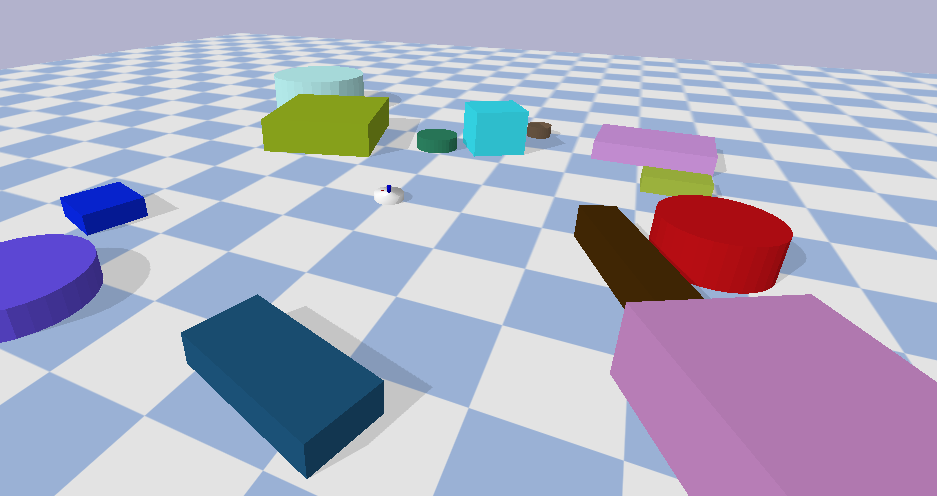
\includegraphics[width=\textwidth]{figures/tests/random1}
    \end{subfigure}
    \hfill
    \begin{subfigure}{.49\textwidth}
    \centering
    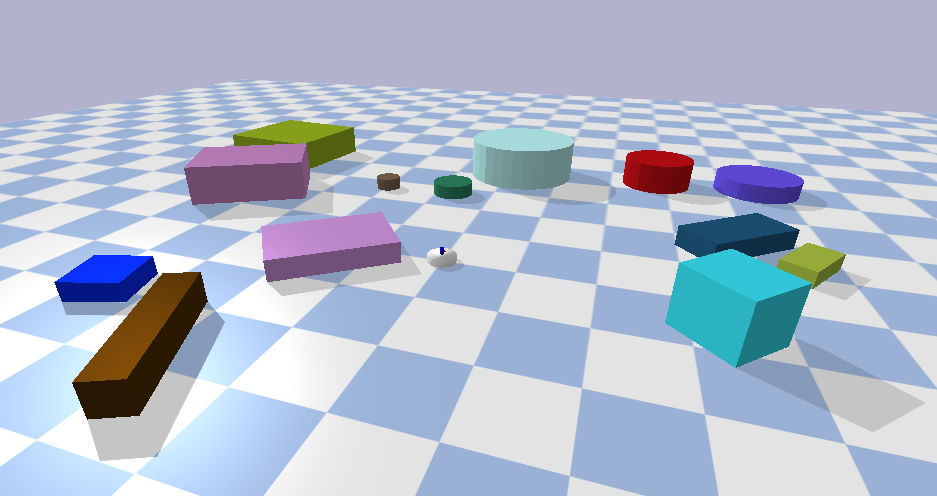
\includegraphics[width=\textwidth]{figures/tests/random2}
    \end{subfigure}

    \vspace{0.2cm}
    \begin{subfigure}{.49\textwidth}
    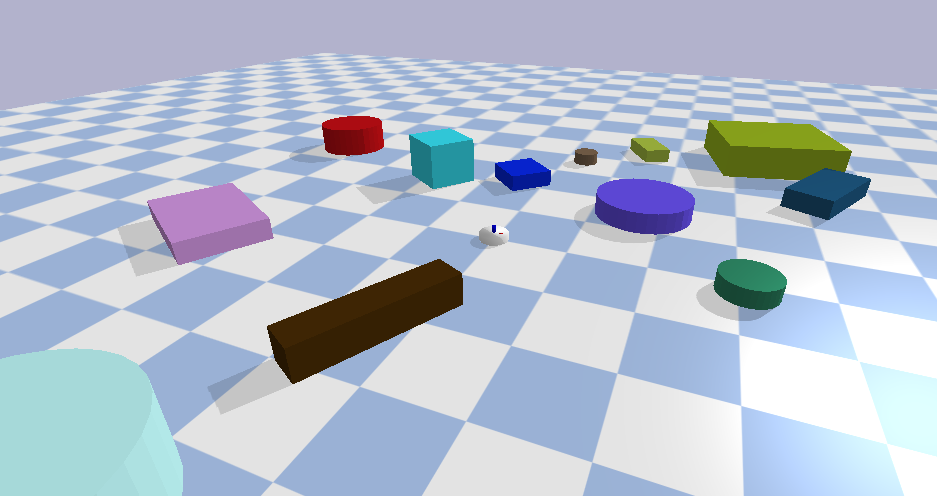
\includegraphics[width=\textwidth]{figures/tests/random3}
    \end{subfigure}
    \hfill
    \begin{subfigure}{.49\textwidth}
    \centering
    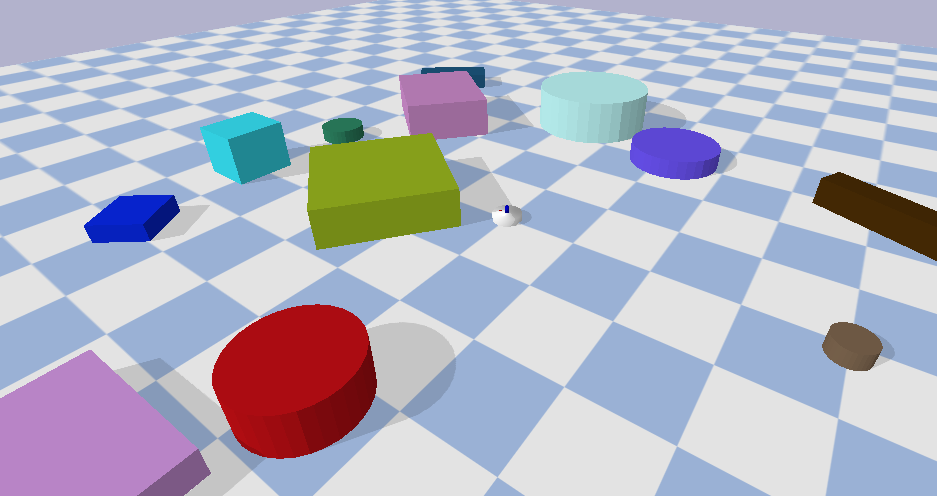
\includegraphics[width=\textwidth]{figures/tests/random4}
    \end{subfigure}
    \caption{A random environment that is reshuffled 4 times. Target ghost configurations are not shown.}
    \label{fig:random_environment_reshuffle}
\end{figure}

The \ac{halgorithm} will be tested with both driving and pushing tasks. Starting with driving tasks for which the parameters are set to be.\bs

\begin{center}
\begin{align*}
\text{grid size} \quad &\gls{x}=12, \quad \gls{y}=12 \\
\text{object size} \quad &\mathit{min\_length}=0.2, \quad \mathit{max\_length}=2 \\
\text{object weight} \quad &\mathit{max\_weight}=1000 \\
\text{number of objects} \quad &\mathit{num\_unmovable\_obj}=3, \quad \mathit{num\_movable\_obj}=5 \\
\text{number of subtasks} \quad &\mathit{num\_subtasks}=3
\end{align*}
\end{center}

These parameters have been specifically selected, starting with the size of the ground floor. The ground floor should be large enough such that objects can be pushed around, note that, for a driving task, pushing is involved when a path must be freed. Environments must thus not be too small. A ground floor too large would result in a longer computational time for path estimation and planning which is undesired. A 12 by 12 is selected because it is reflecting a reasonably large workspace, whilst computation times for planning are kept similar to computation times. The range that determines the size of objects is set such that objects can be as large as the robot itself, and be around 10 times as large as the robot. With these sizes the robot is unable to grasp objects, a gripper would be too small to grasp objects. The comparatively large size fits the objective of nonprehensile pushing, there simply is no other method to manipulate such large objects other than pushing. A real-life example are can be found in harbours where tug boats push giant cargo ships around that are many times over the size of the tug boat. The ratio of solid obstacles vs.~movable objects determines if a task is more navigation (only solid obstacles) or more \ac{NAMO} (only movable objects). A task that tends toward \ac{NAMO} is favoured because that is the target environment in this thesis. There should be some unmovable obstacles that reward the robot learning such objects are unmovable (to then not interact with them). Thus there are more movable objects than solid obstacles chosen, whilst still having 2 solid obstacles around. The number of subtasks is set to 3, a low number of drive subtasks that can be completed in under 2 minutes.\bs

The following figure shows a driving task containing 3 subtasks for the robot, which translates into driving to three target configurations. The randomly generated task in the random environment is reshuffled and then solved 10 times. The sequence of tasks is performed with the \ac{kgraph} suggestions. 

\begin{figure}[H]
    \centering
    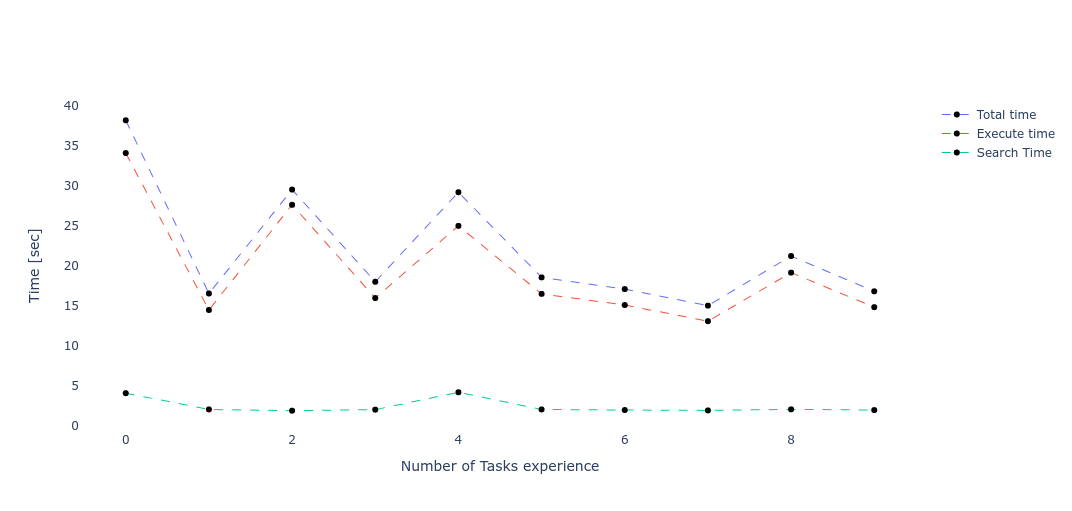
\includegraphics[width=0.9\textwidth]{figures/results/random_drive_execution_times}
    \caption{Robot tasked to drive toward 3 target configurations, the environment is reshuffled after completing a task.}%
    \label{fig:rand_drive_times}
\end{figure}

What is not shown in the above figure is that the \ac{kgraph} over times prefers the \ac{MPC} controller over the \ac{MPPI} controller (both using the \textit{lti-model-1}) because of its lower average prediction error. The \ac{MPC} controller is a bit faster compared to the \ac{MPPI} controller thus the execution time decreases over time. The execution time is strongly correlated with the path length because driving to a target further away takes longer. It is thus only useful to investigate the trend that \Cref{fig:rand_drive_times} and not individual data points.\bs

Then the same environments and tasks are solved 10 times without the \ac{kgraph} suggestions. The randomly generated tasks and environments are repeatable by fixing the seed. The fixed seed ensures that the randomly generated environments can be created multiple times, once to solve with \ac{kgraph} suggestions and once to solve without help from the \ac{kgraph}.\bs

\begin{figure}[H]
    \centering
    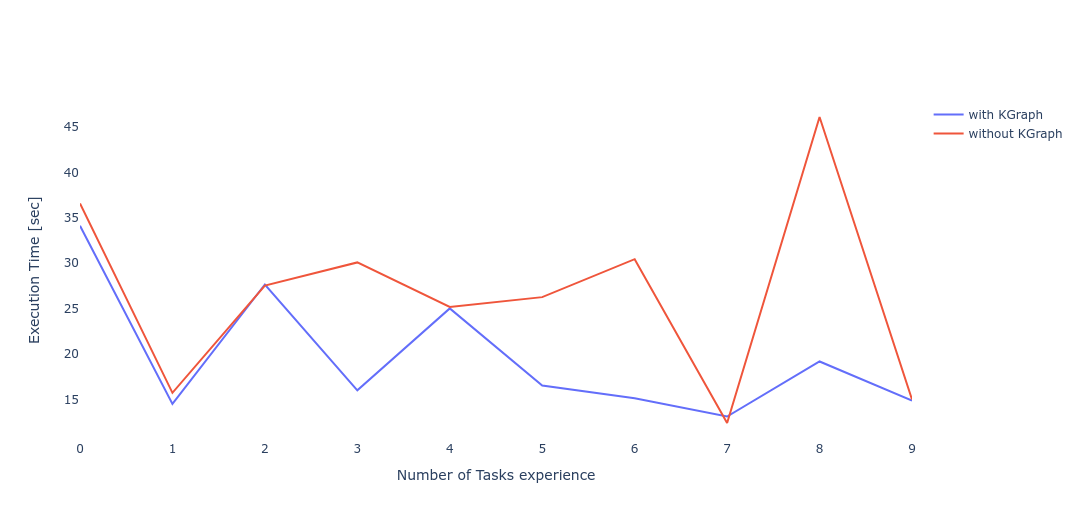
\includegraphics[width=0.9\textwidth]{figures/results/random_drive_with_without_kgraph}
    \caption{Execution times for driving toward target configurations with and without \ac{kgraph}.}%
    \label{fig:results_random_drive_task}
\end{figure}

The figure above shows similar running times at the first few solved tasks. During these first tasks the \ac{kgraph} is filled with edge feedback, but the \ac{kgraph} has not gained enough feedback to suggest action parameterizations, this period can be referred to as the learning phase. After this learning phase, the \ac{kgraph} suggests the \ac{MPC} controller over the \ac{MPPI} controller, because of its relatively higher \textit{success factor}. The action suggestions improve overall execution time, note that selecting random controllers can result in equal execution time. In these cases, (4, 7 or 9 tasks in experience in \cref{fig:results_random_drive_task}) the randomly selected controllers all were \ac{MPC} controllers.\bs

Now the \ac{halgorithm} is tasked with pushing a single object toward a target configuration. Except for the number of subtasks all parameters that determine the random environment will remain as previously set for the random driving task.\bs

\begin{figure}[H]
    \centering
    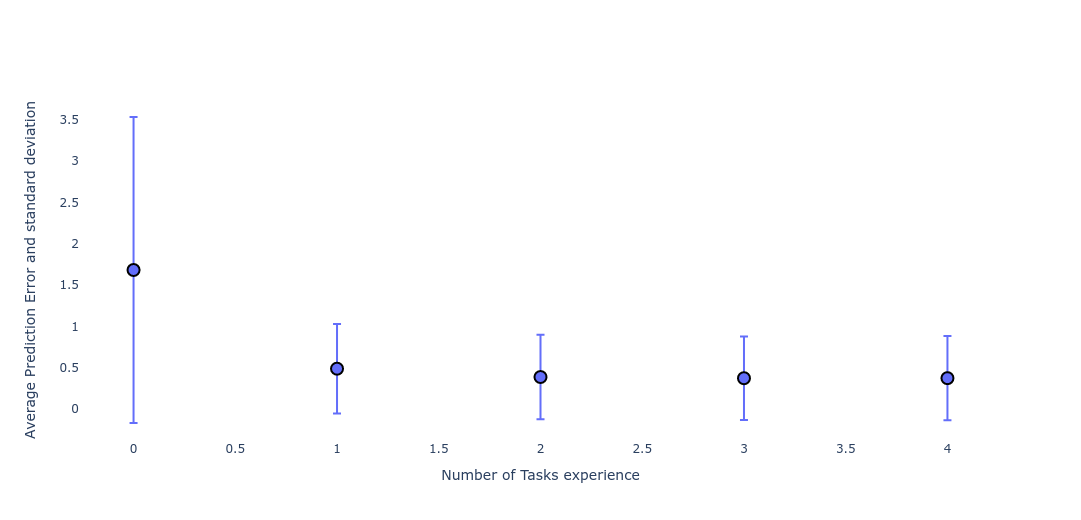
\includegraphics[width=0.9\textwidth]{figures/results/rand_push_pred_error}
    \caption{Average Prediction Error and Standard Deviation for action edges during a pushing task.}%
    \label{fig:rand_push_full_pred}
\end{figure}

The \ac{MPPI} controller with \textit{nonlinear-push-model-1} has an average \ac{PE} between 1.5 and 2 and can be seen in the figure above as the most left data point in the prediction error plot. The same controller with \textit{nonlinear-push-model-2} has an average lower \ac{PE} between 0.4 and 0.6 and can be seen in the following data points (1, 2, 3 and 4). The \textit{success factor} is calculated based on the average prediction error so it is expected that the \ac{kgraph} suggests the controller with the lower prediction error. It is expected that the \ac{PE} goes down, which is exactly what \Cref{fig:rand_push_full_pred} shows. The \ac{halgorithm} tests both edge parameterisations to conclude that the \ac{MPPI} controller and \textit{nonlinear-push-model-2} is the better of the two.  

\begin{figure}[H]
    \centering
    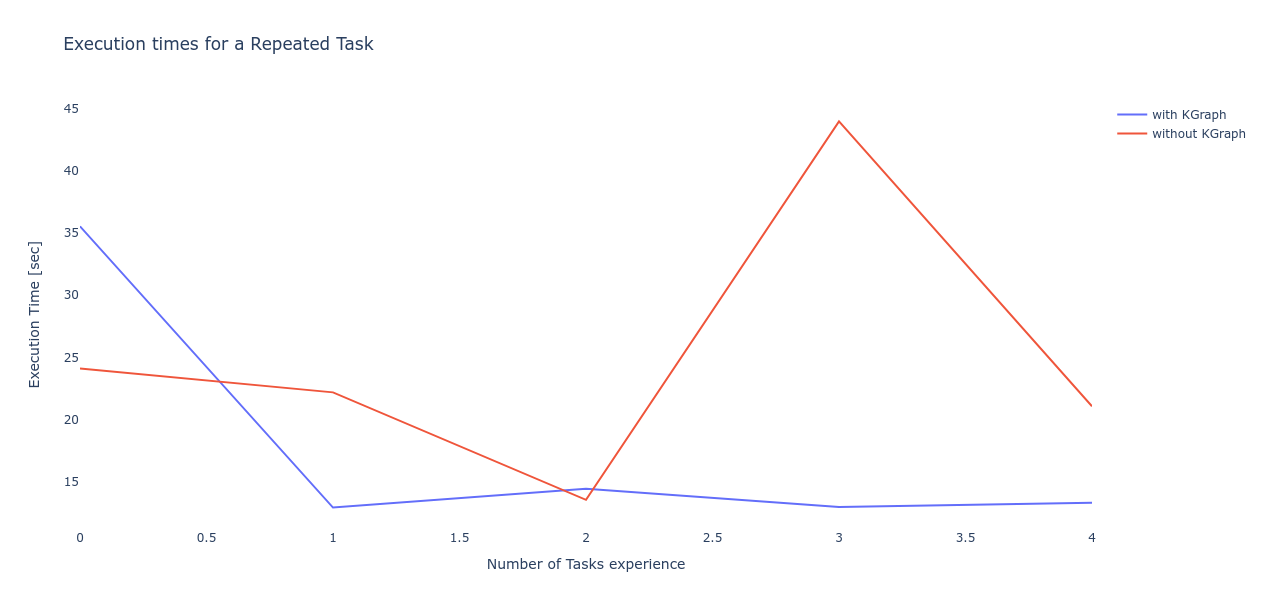
\includegraphics[width=0.9\textwidth]{figures/results/random_push_execution_times}
    \caption{Planning times for pushing an object toward the target a configuration.}%
    \label{fig:random_push_all_times}
\end{figure}

The \ac{MPPI} controller with \textit{nonlinear-push-model-2} does not only have a lower \ac{PE} but is also faster compared to the \ac{MPPI} controller combined with \textit{nonlinear-push-model-1}. Execution time for driving toward the object and pushing that object to its target location takes around 15 seconds, with a search time to find that hypothesis being between 10 to 15 seconds. The result is that task execution time lowers, bear in mind that this result has to be taken with a grain of salt because the execution time is correlated with the path length (how far the object is from the robot, and how far should the object be pushed). It is better to look at the figure below that displays the execution time of both solving the same task with help of the \ac{kgraph} and without its help.

\begin{figure}[H]
    \centering
    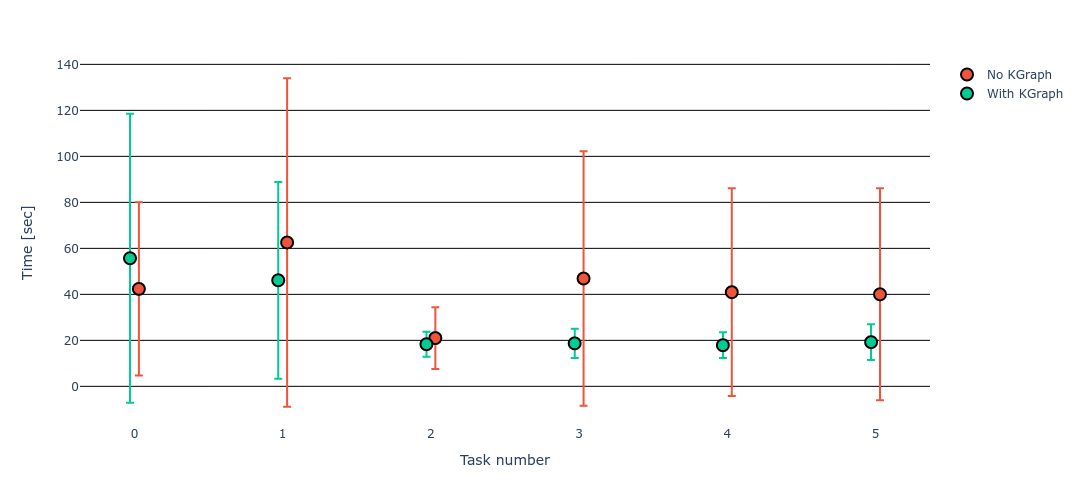
\includegraphics[width=0.9\textwidth]{figures/results/random_push_with_without_kgraph}
    \caption{Execution times for pushing an object to target configurations with and without \ac{kgraph}.}%
    \label{fig:random_push_with_without_kgraph}
\end{figure}

The \ac{kgraph} suggestion work in favour of the execution time as can be seen in the \Cref{fig:random_push_with_without_kgraph}. Noticable is that a random selection by pure change selects the best choice of the controller as can be seen in 2 tasks of experience in the figure above.

% \section{Knowledge Graph On/Off}%
% \label{sec:kgraph_on_off}
% Influence of the \ac{kgraph} is shown using the random environment. The robot will once complete many random tasks with the help of \ac{kgraph} and once the robot will complete many random tasks without the help of \ac{kgraph}. The results can be compared in \Cref{fig:results_random_kgraph_on_off}.\bs
%
% \begin{figure}[H]
%     \centering
%     
\includegraphics[width=0.9\textwidth]{figures/tests/404_not_found}
%     \caption{Some test are still under development for the randomization where the kgraph is once on and once off.}%
%     \label{fig:results_random_kgraph_on_off}
% \end{figure}
%
% \todo[inline]{Test to create results for running (run that many times) the random environment}
%

\section{Comparison with State-of-the-Art}%
\label{sec:compare_with_related_papers}

In the introduction \Cref{table:sota_and_3_topics} was presented. A table that mainly shows which subset of the 3 main topics are included in which scientific paper. The 3 topics are learning system models, the \ac{NAMO} problem and nonprehesile pushing. The table is presented again with the addition of the main testing method that is used by the state-of-the-art paper.

\noindent
\begin{table}[H]
  \centering
  \rowcolors{2}{white}{myEvenLighterColor}
  \begin{tabular}
  {>{\raggedright\arraybackslash}P{1.8cm}%
    >{\raggedleft\arraybackslash}P{1.4cm}%
    >{\raggedright\arraybackslash}P{1.2cm}%
    >{\raggedright\arraybackslash}P{1.2cm}%
    >{\raggedright\arraybackslash}P{1.2cm}%
    >{\raggedright\arraybackslash}P{1.6cm}
    >{\raggedright\arraybackslash}P{3.8cm}
  }
  Author & Citation & Learns\newline object\newline dynamics & \ac{NAMO} & Specify object target positions & Object\newline Manipu- lation & test metric\\
  \citeauthor{ellis_navigation_2022} &\cite{ellis_navigation_2022} & \cmark& \cmark& \xmark& pushing & \underline{success rate}\\
\citeauthor{sabbaghnovin_model_2021} &\cite{sabbaghnovin_model_2021} & \cmark& \xmark& \cmark& grasp-push grasp-pull & success rate, \underline{execution time} \underline{prediction error}, final position error \\
\citeauthor{scholz_navigation_2016} &\cite{scholz_navigation_2016} & \cmark& \cmark& \xmark& graph-push grasp-pull & runtime, planning time, \underline{number of calls to planner} number of calls to update model\\
\citeauthor{vega-brown_asymptotically_2020} &\cite{vega-brown_asymptotically_2020} & \xmark& \cmark& \cmark& gripping & \underline{computation time}\\
\citeauthor{wang_affordancebased_2020} &\cite{wang_affordancebased_2020} & \cmark& \cmark& \xmark& pushing & \underline{computation and} \underline{execution time}\\
    Groote & proposed solution &  \xmark/\cmark& \cmark& \cmark& pushing & see \Cref{table:proposed_method_metrics}\\
  \end{tabular}
  \caption{Overview of recent state-of-the-art papers that include a subset of the 3 topics (learning system models, \ac{NAMO}, and nonprehensile pushing). The \textit{grasp-push} and \textit{grasp-pull} refer to prehensile push and pull manipulation, \textit{gripped} refers to fully gripping and lifting objects for manipulation, \textit{pushing} refers to nonprehensile push manipulation. The test metric indicates the testing method used by the paper, where the underlined metric is used to compare against the proposed method.}%
\label{table:sota_vs_results_proposed method}
\end{table}

\paragraph{Comparing Success Rate}
\citeauthor{ellis_navigation_2022} claims to push with a success rate of a 100\%~\cite{ellis_navigation_2022}. The test environment that \citeauthor{ellis_navigation_2022} has used is very similar to the random pushing task discussed in \Cref{sec:randomisation}. For both the random driving task and the random pushing task the success rate is 100\%. Meaning that every driving or pushing subtask was successfully completed. It is even so that for the result of the random push task (displayed in \Cref{fig:rand_push_full_pred,fig:random_push_all_times,fig:random_push_with_without_kgraph}) the number of hypotheses is equal to the number of subtasks. Meaning that every subtask is completed by the first hypothesis generated. Both similar experiments from \citeauthor{ellis_navigation_2022} and this thesis have a 100\% success rate for similar 
, allowing us to conclude that the results are comparable.

\paragraph{Comparing Computation and Execution Time}
Three state-of-the-art papers that use computation and execution time as the testing metrics are compared to the proposed method. To accomplish a fair comparison the environments that have been used in the citations are rebuilt in the pybullet software. The results are then directly compared to conclude that the proposed method is as good as or even better in terms of computation time and execution time for similar tasks.\bs

\citeauthor{wang_affordancebased_2020} drives toward a target configuration that is blocked by a chair. The task is performed 3 times where the robot may remember its interactions with the chair from previous runs. The task is successfully completed all three times with a total time of 200 seconds for the first run to 180 seconds for the third run. Execution time increased from 70 to 85 seconds during these runs. Even with increasing execution times, the solution is found faster because the experience from previous runs could be used that lowered search time~\cite{wang_affordancebased_2020}. To compare against these results the environment is recreated in the pybullet software. The proposed method was run only once, during this run it classified a wall object as unmovable, and the pushable box object with dimensions equal to that of the chair was classified as movable and moved out of the way. Overall execution time was 45 seconds whilst computation time took 65 seconds. The proposed method successfully completed this similar task whilst having a lower computation and execution time. This allows concluding that the proposed method improves upon the paper from \citeauthor{wang_affordancebased_2020} with a decent margin.\bs

\citeauthor{vega-brown_asymptotically_2020} has a task that pushes two boxes into a goal region. It takes around 300 seconds to return a hypothesis~\cite{vega-brown_asymptotically_2020}. Both pushing tasks can be compared with two separate pushing tasks from the random push environment. By doubling the time to push a single object to its target configuration, $2 \cdot 30 = 60$ seconds both tasks could be compared. However, the point of \citeauthor{vega-brown_asymptotically_2020} paper is that a global minimal task is sought. The proposed method randomly selects a subtask and tries to complete it to then move to the next randomly selected subtask. A global minimum is thus not sought and both papers can therefore not be compared properly.\bs

\citeauthor{sabbaghnovin_model_2021} grasp-pushes and grasp-pulls a walker object to two new target configurations~\cite{sabbaghnovin_model_2021}. The task is mimicked by pushing a box object of equal dimensions to the same target configurations. Compared to \citeauthor{sabbaghnovin_model_2021} average of 125 and 160 seconds to complete task 1 and task 2 the proposed method takes an average of only 27 and 33 seconds respectively (10 seconds computation time) to complete similar tasks. The decrease in total time allows to conclude that the proposed methods improve upon the method proposed by~\citeauthor{sabbaghnovin_model_2021}.\bs

\paragraph{Comparing Prediction Error}
\citeauthor{sabbaghnovin_model_2021} displays the final position errors for a selection of objects which range from 0.05 to 0.6 meters. A success threshold is set to 0.1 meters, which determines that the object is at its target location~\cite{sabbaghnovin_model_2021}. The success threshold in this thesis is set to a staggering 0.9 meters, thus it is concluded an object has reached its target position, whilst it is still 0.9 meters from its target configurations. This thesis does not try to reach optimal control, it tries to select the best controller in the available set of controllers. If the same controller from \citeauthor{sabbaghnovin_model_2021} would be available, then similar final position errors would be obtained. It can be concluded that the prediction error of the proposed method is worse compared to this state-of-the-art method. The reason is that the proposed method focuses on improving the control selection and action sequences over time, and not on lowering final prediction errors.\bs 

% \paragraph{Comparing Number of Replanning times}
% \todo[inline]{\cite{scholz_navigation_2016}}
